% Copyright 2024 Louis Paternault
%
% This file is part of pdfimpose-web.
%
% Pdfimpose-web is free software: you can redistribute it and/or modify it
% under the terms of the GNU Affero General Public License as published by the
% Free Software Foundation, either version 3 of the License, or (at your
% option) any later version.
%
% Pdfimpose-web is distributed in the hope that it will be useful, but WITHOUT
% ANY WARRANTY; without even the implied warranty of MERCHANTABILITY or FITNESS
% FOR A PARTICULAR PURPOSE. See the GNU Affero General Public License for more
% details.
%
% You should have received a copy of the GNU Affero General Public License
% along with pdfimpose-web. If not, see <https://www.gnu.org/licenses/>.

\documentclass[tikz]{standalone}

\renewcommand{\familydefault}{\sfdefault}

\begin{document}

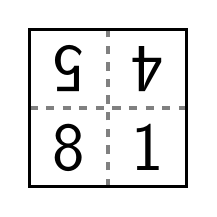
\begin{tikzpicture}[every node/.style={font=\Huge}]
  \draw[very thick, dashed, gray] (.5, -.5) -- ++(0, 2);
  \draw[very thick, dashed, gray] (-.5, .5) -- ++(2, 0);
  \draw[very thick] (-.5, -.5) rectangle (1.5, 1.5);
  \draw (0, 0) node{8};
  \draw (1, 0) node{1};
  \draw (0, 1) node[rotate=180]{5};
  \draw (1, 1) node[rotate=180]{4};
\end{tikzpicture}

\end{document}
